\documentclass{beamer}
\mode<presentation>
{
  \usetheme{Warsaw}
  \definecolor{mcgarnet}{rgb}{0.38, 0, 0.08}
  \definecolor{mcgray}{rgb}{0.6, 0.6, 0.6}
  \setbeamercolor{structure}{fg=mcgarnet,bg=mcgray}
  %\setbeamercovered{transparent}
}


\usepackage[english]{babel}
\usepackage[latin1]{inputenc}
\usepackage{times}
\usepackage[T1]{fontenc}
\usepackage{tikz}
\usepackage{graphicx}
\usepackage{xcolor}

\newcommand{\imagesource}[1]{{\centering\hfill\break\hbox{\scriptsize Image Source:\thinspace{\small\itshape #1}}\par}}

\title{Significant Figures and Rounding}


\author{Robert Lowe\\}

\institute[Maryville College] % (optional, but mostly needed)
{
  Division of Mathematics and Computer Science\\
  Maryville College
}

\date[]{}
\subject{}

\pgfdeclareimage[height=0.5cm]{university-logo}{images/Maryville-College}
\logo{\pgfuseimage{university-logo}}



\AtBeginSection[]
{
  \begin{frame}<beamer>{Outline}
    \tableofcontents[currentsection]
  \end{frame}
}


\begin{document}

\begin{frame}
  \titlepage
\end{frame}

\begin{frame}{Outline}
  \tableofcontents
\end{frame}


% Structuring a talk is a difficult task and the following structure
% may not be suitable. Here are some rules that apply for this
% solution: 

% - Exactly two or three sections (other than the summary).
% - At *most* three subsections per section.
% - Talk about 30s to 2min per frame. So there should be between about
%   15 and 30 frames, all told.

% - A conference audience is likely to know very little of what you
%   are going to talk about. So *simplify*!
% - In a 20min talk, getting the main ideas across is hard
%   enough. Leave out details, even if it means being less precise than
%   you think necessary.
% - If you omit details that are vital to the proof/implementation,
%   just say so once. Everybody will be happy with that.

\section{Rounding}
\begin{frame}{When to Round}
\begin{itemize}[<+->]
    \item Estimation
    \item Significant Digits in Measurements
    \item When it makes sense for units (for instance, in money).
\end{itemize}
\end{frame}

\begin{frame}{Rounding Method}
\begin{enumerate}[<+->]
    \item Choose a digit to round to.
    \item Look to the digit to the right of this one.
    \item If the digit is $\geq 5$, add 1 to the digit you are rounding to.
    \item The digits to the right of this position become zero.
\end{enumerate}
\end{frame}

\begin{frame}{Examples}
Round the following to the 10's place:
\begin{enumerate}
    \item<1-> 12.5 \uncover<2->{\textcolor{green}{$10$}}
    \item<3-> 17.9 \uncover<4->{\textcolor{green}{$20$}}
    \item<5-> 14.999 \uncover<6->{\textcolor{green}{$10$}}
\end{enumerate}
\end{frame}

\begin{frame}{Examples}

Round the following to the 100's place:
\begin{enumerate}
    \item<1-> 125 \uncover<2->{\textcolor{green}{$100$}}
    \item<3-> 170 \uncover<4->{\textcolor{green}{$200$}}
    \item<5-> 14 \uncover<6->{\textcolor{green}{$0$}}
\end{enumerate}
\end{frame}


\begin{frame}{Examples}

Round the following to 1/10th's place
\begin{enumerate}
    \item<1-> 12.54555 \uncover<2->{\textcolor{green}{12.5}}
    \item<3-> 12.78 \uncover<4->{\textcolor{green}{12.8}}
    \item<5-> 1.31111 \uncover<6->{\textcolor{green}{1.3}}
\end{enumerate}
\end{frame}

\section{Significance}
\begin{frame}{Accuracy and Precision}
\begin{itemize}[<+->]
    \item A number by itself is an abstract (or exact) number.
    \item A number which quantifies objects or units is a concrete number.
    \item A measurement is a number observed using some instrument (ruler, scale, etc.).
    \item Measurements will always contain errors.
    \item {\bf Accuracy} - The distance between an observed value and the actual value.
    \item {\bf Precision} - The distance between repeated observations.
\end{itemize}
\end{frame}

\begin{frame}{Significant Digits}
\begin{itemize}[<+(1)->]
    \item Significant digits roughly correspond to the precision of the instrument used to take measurements. 
    \item When performing calculations, your answer cannot be more precise than your measurements!
\end{itemize}

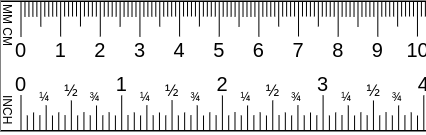
\includegraphics[height=1in]{../lectures/images/ruler-4-1875in}
\end{frame}

\begin{frame}{Significant Digit Rules}
\begin{enumerate}[<+->]
    \item All non-zero digits are significant.
    \item Any zero digits between significant digits are significant.
    \item A trailing zero is significant only if it appears to the right of the decimal point.
\end{enumerate}
\end{frame}

\begin{frame}{Examples}

How many significant digits are in each of the following?\newline
\begin{enumerate}
    \item<1-> 1 \uncover<2->{\textcolor{green}{1 significant digit}}
    \item<3-> 10 \uncover<4->{\textcolor{green}{1 significant digit}}
    \item<5-> 1.0 \uncover<6->{\textcolor{green}{2 significant digits}}
    \item<7-> 10.0 \uncover<8->{\textcolor{green}{3 significant digits}}
    \item<9-> 0.000312 \uncover<10->{\textcolor{green}{3 significant digits}}
    \item<11-> 0.00300 \uncover<12->{\textcolor{green}{3 significant digits}}
\end{enumerate}
\end{frame}


\begin{frame}{Addition with Significant Digits}
\begin{enumerate}[<+->]
    \item Count the number of significant digits to the right of the decimal place in each of the numbers you are adding. This is the number of significant digits that your answer can have to the right of the decimal place.
    \item Add as normal.
    \item Round the sum to the correct number of significant digits.
\end{enumerate}
\end{frame}


\begin{frame}{Multiplication with Significant Digits}
\begin{enumerate}[<+->]
    \item Count the number of significant digits in each number you are multiplying. This is the number of significant digits that can be in your answer.
    \item Multiply as normal.
    \item Round the product to the correct number of significant digits.
\end{enumerate}
\end{frame}

\begin{frame}{Examples}
\begin{enumerate}
    \item<1-> $10\mathrm{in} + 11\mathrm{in} = ?$
        \uncover<2->{\textcolor{green}{21in}}
    \item<3-> $1\mathrm{mm} + 2.0\mathrm{mm} = ?$ 
        \uncover<4->{\textcolor{green}{3mm}}
    \item<5-> $1.125\mathrm{kg} + 0.1\mathrm{kg} = ?$
        \uncover<6->{\textcolor{green}{1.2kg}}
    \item<7-> $1.5\mathrm{in} \times 2.125\mathrm{in} = ?$ 
        \uncover<8->{\textcolor{green}{$3.2\mathrm{in^2}$}}
    \item<9-> $10.0\mathrm{mm} \times 2\mathrm{mm} = ?$
        \uncover<10->{\textcolor{green}{$20\mathrm{mm^2}$}}
    \item<10-> Compute the Perimeter of your student ID.
    \item<11-> Compute the area of your student ID.
\end{enumerate}
\end{frame}

\begin{frame}{Significant Digits and Scientific Notation}
When using scientific notation, only write significant digits.
\end{frame}

\begin{frame}{When to Use Significant Digits}
Significant digit considerations only apply to values observed via
measurement.  They do not apply to counting, abstract numbers, or
theoretical values.
\end{frame}


\end{document}
